%% ergebnisse.tex

\chapter{Ergebnisse und Diskussion}
\label{ch:Ergebnisse}

\section{Allgemeine Merkmale des Netzwerkes}
\label{sec:result-allg-merkm-des}

\section{Eigenschaften einzelner Schl\"ussel}
\label{sec:result-key-properties}

\section{Struktur der starken Zusammenhangskomponenten}
\label{sec:result-komponentenstruktur}

\begin{figure}[h]
  \centering
  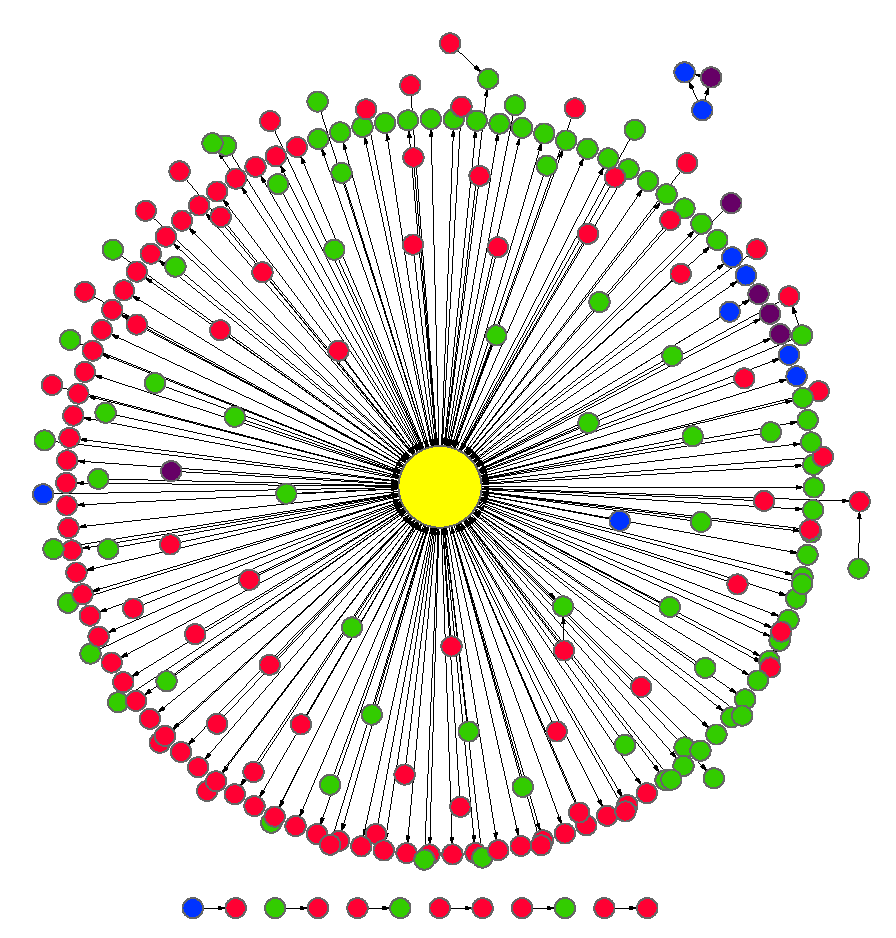
\includegraphics[scale=1.0]{images/component-metagraph-8.pdf}
  \caption{Struktur der starken Zusammenhangskomponenten bis zur
    Grösse 6 (rot = Grösse 6-10, grün = Grösse 11-20, blau = Grösse
    21-30, violett = Grösse $>= 31$, gelb = MSCC)}
  \label{fig:komponenten-struktur}
\end{figure}

\section{Zusammenhangskomponenten und Communities}
\label{sec:result-zusamm-und-comm}

\begin{figure}[h]
  \centering
  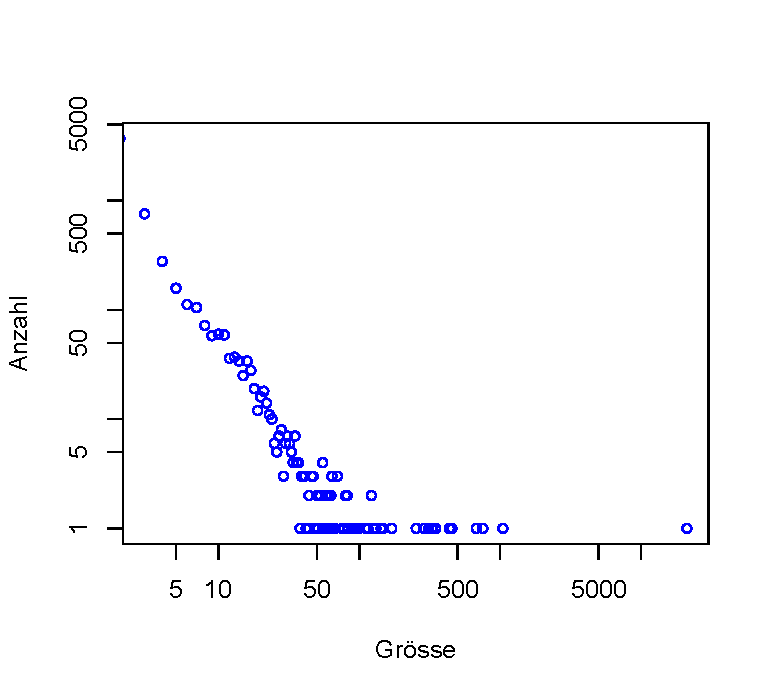
\includegraphics[scale=0.8]{images/community-size-dist.pdf}
  \caption{Gr\"ossenverteilung der von Fast-Modularity (FASTMOD),
    Label-Propagation (LABELPROP) und COPRA berechneten Communities}
  \label{fig:community-size-dist}
\end{figure}

\begin{table}[h]
  \centering
  \begin{tabular}{l|c|p{4cm}|p{4cm}}
    Algorithmus & Modularity & Anzahl Communities (Gr\"osse $> 3$) &
    Anzahl enthaltener Knoten \\
    \hline
    fastmod & 0,596 & 552 & foo \\
    labelprop & 0,658 & 1834 & foo \\
    cliquemod-3000 & 0,670 & 811 & foo \\
    cliquemod-500 & 0,677 & 451 & foo \\
    copra & --- & 1354 & foo
  \end{tabular}
  \caption{Modulairty, Anzahl communities, Menge enthaltener Knoten (> 3)}
  \label{tab:foo}
\end{table}

{\footnotesize
\begin{table}[h]
  \centering
  \begin{tabular}{l|c|c|c|c|c|c}
    Algo & TLD-S & TLD-M & SLD-S & SLD-M & SIG \\
    \hline
    fastmod & 293 (53\%) & 247 (44\%) & 66 (11\%) & 194 (35\%) & 128
    (23\%) \\
    \hline
    labelprop & 1048 (57\%) & 755 (41\%) & 277 (15\%) & 720 (39\%) &
    553 (30\%) \\
    \hline
    cliquemod-3000 & 460 (56\%) & 332 (40\%) & 104 (12\%) & 300 (36\%)
    & 230 (28\%) \\
    \hline
    cliquemod-500 & 230 (50\%) & 209 (46\%) & 65 (14\%) & 141 (31\%) &
    116 (25\%) \\
    \hline
    copra & 792 (58\%) & 525 (38\%) & 259 (19\%) & 533 (39\%) & 555 (40\%)

  \end{tabular}
  \caption{SLD-TLD-Zuweisung, TIME-CORR}
  \label{tab:assign}
\end{table}
}

\begin{figure}[t]
  \centering
  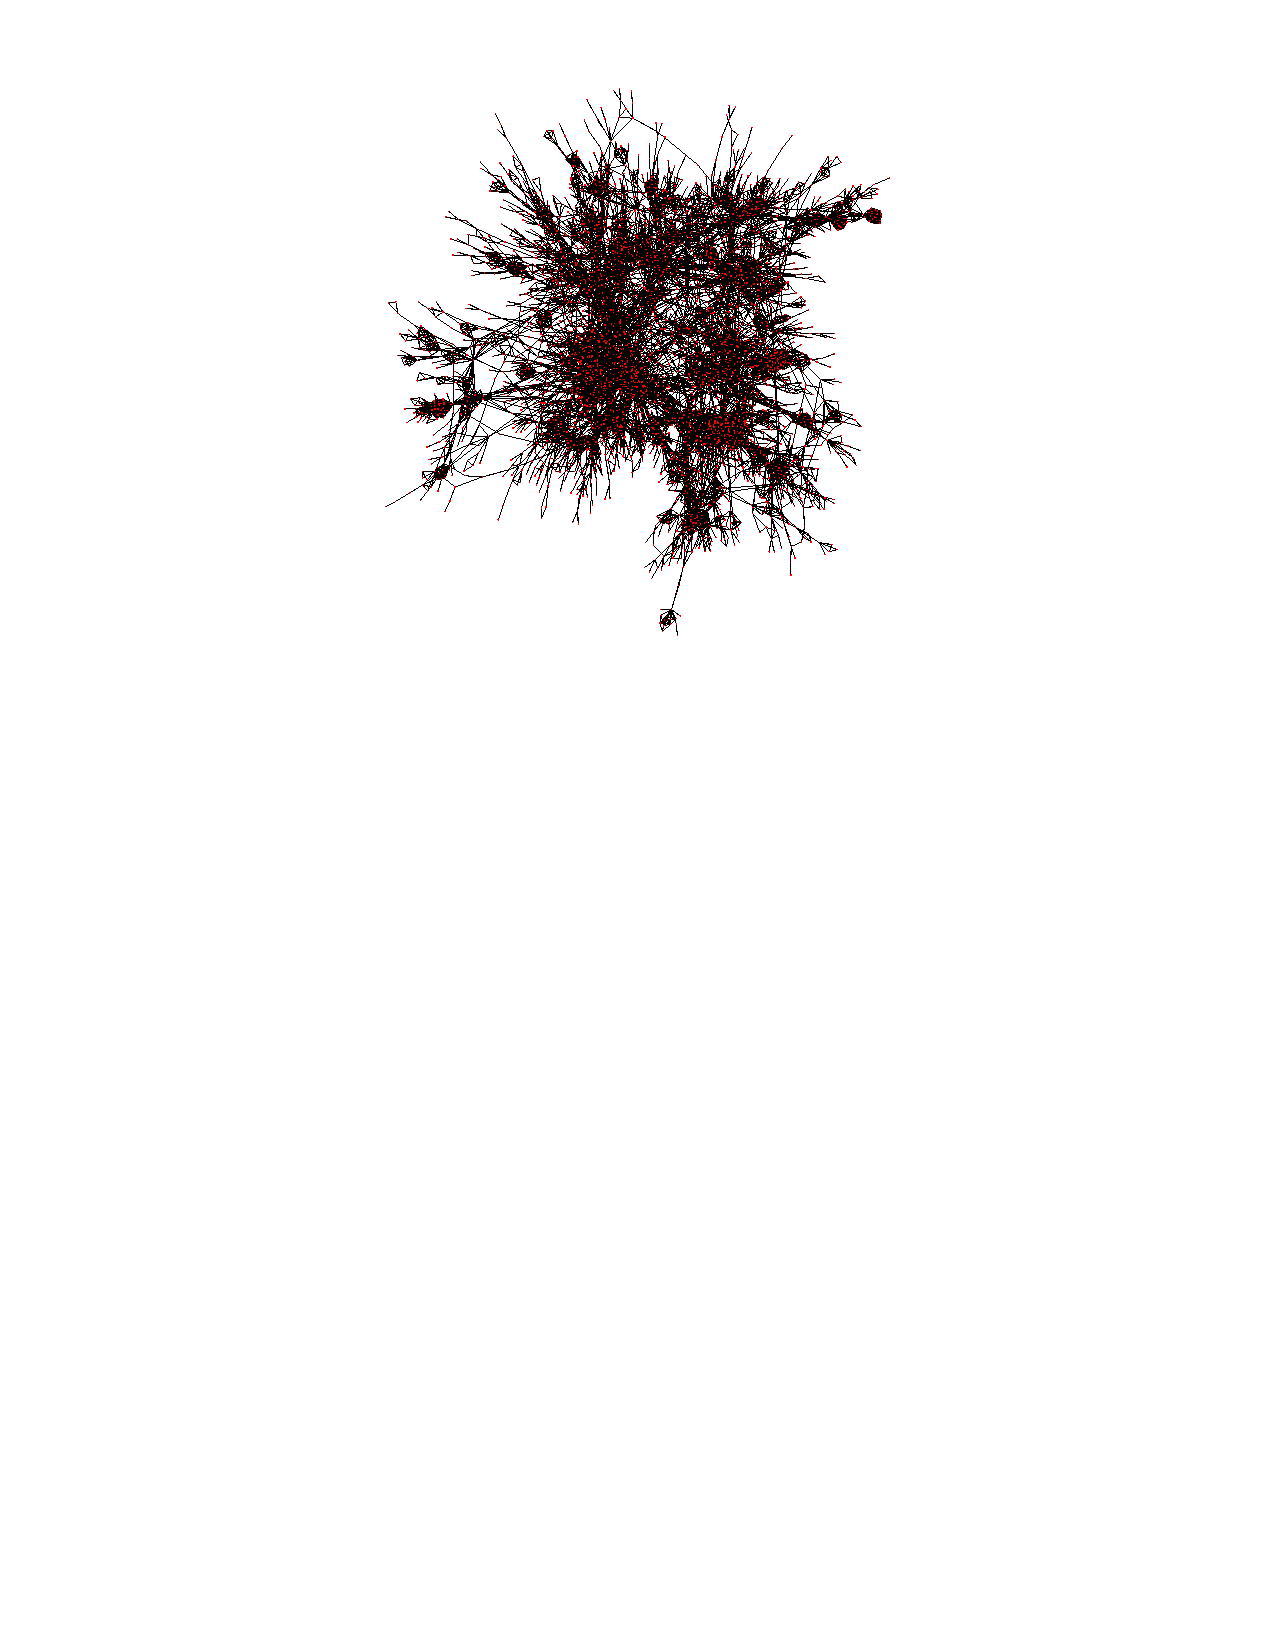
\includegraphics[scale=1.7]{images/fastmod-subgraph-large-modular-6525064ccab580a0b304a3620b197d7a.pdf}
  \caption{Grosse Community mit modularer Struktur (Berechnet mit
    Fast-Modularity, Force-directed layout)}
  \label{fig:large-community-modular}
\end{figure}

Communities k\"onnen sich nicht nur \"uberlappen. Genauso k\"onnen
einzelne Communities intern wieder eine modulare Struktur haben, so
dass sie sich in mehrere Communities zerlegen lassen.
Abb. \ref{fig:large-community-modular} illustriert, dass die
Verwendung von Methoden zur Berechnung \"uberlappender Communities
sinnvoll sein kann. In der Zeichnung des induzierten Teilgraphen einer
grossen Community (4767 Knoten) aus der
Fast-Modularity-Partitionierung sind etliche dicht gezeichnete
Zusammenballungen von Knoten zu sehen, die nur wenige Kanten nach
aussen haben. Diese k\"onnen als Community-artige Strukturen
interpretiert werden. Zwar kann argumentiert werden, dass die
Zeichnung die Struktur des Teilgraphen nicht notwendigerweise sinnvoll
wiedergibt, dass also die dichten Teilbereiche in der Zeichnung nur
Artefakte der Zeichenmethode darstellen. Allerdings zeigt Noack, dass
starke \"Ubereinstimmungen zwischen einer energieoptimalen Einbettung
eines Graphen in die Ebene nach der Force-directed-Methode und einer
Partitionierung eines Graphen mit optimaler Modularity bestehen
\cite{Noack2009}. Es scheint daher gerechtfertigt, eine Zeichnung
eines Graphen (Force-directed) mit markanten dichten Bereichen als
Indiz f\"ur eine modulare Struktur dieses Graphen zu betrachten.
\begin{figure}[h]
  \centering
  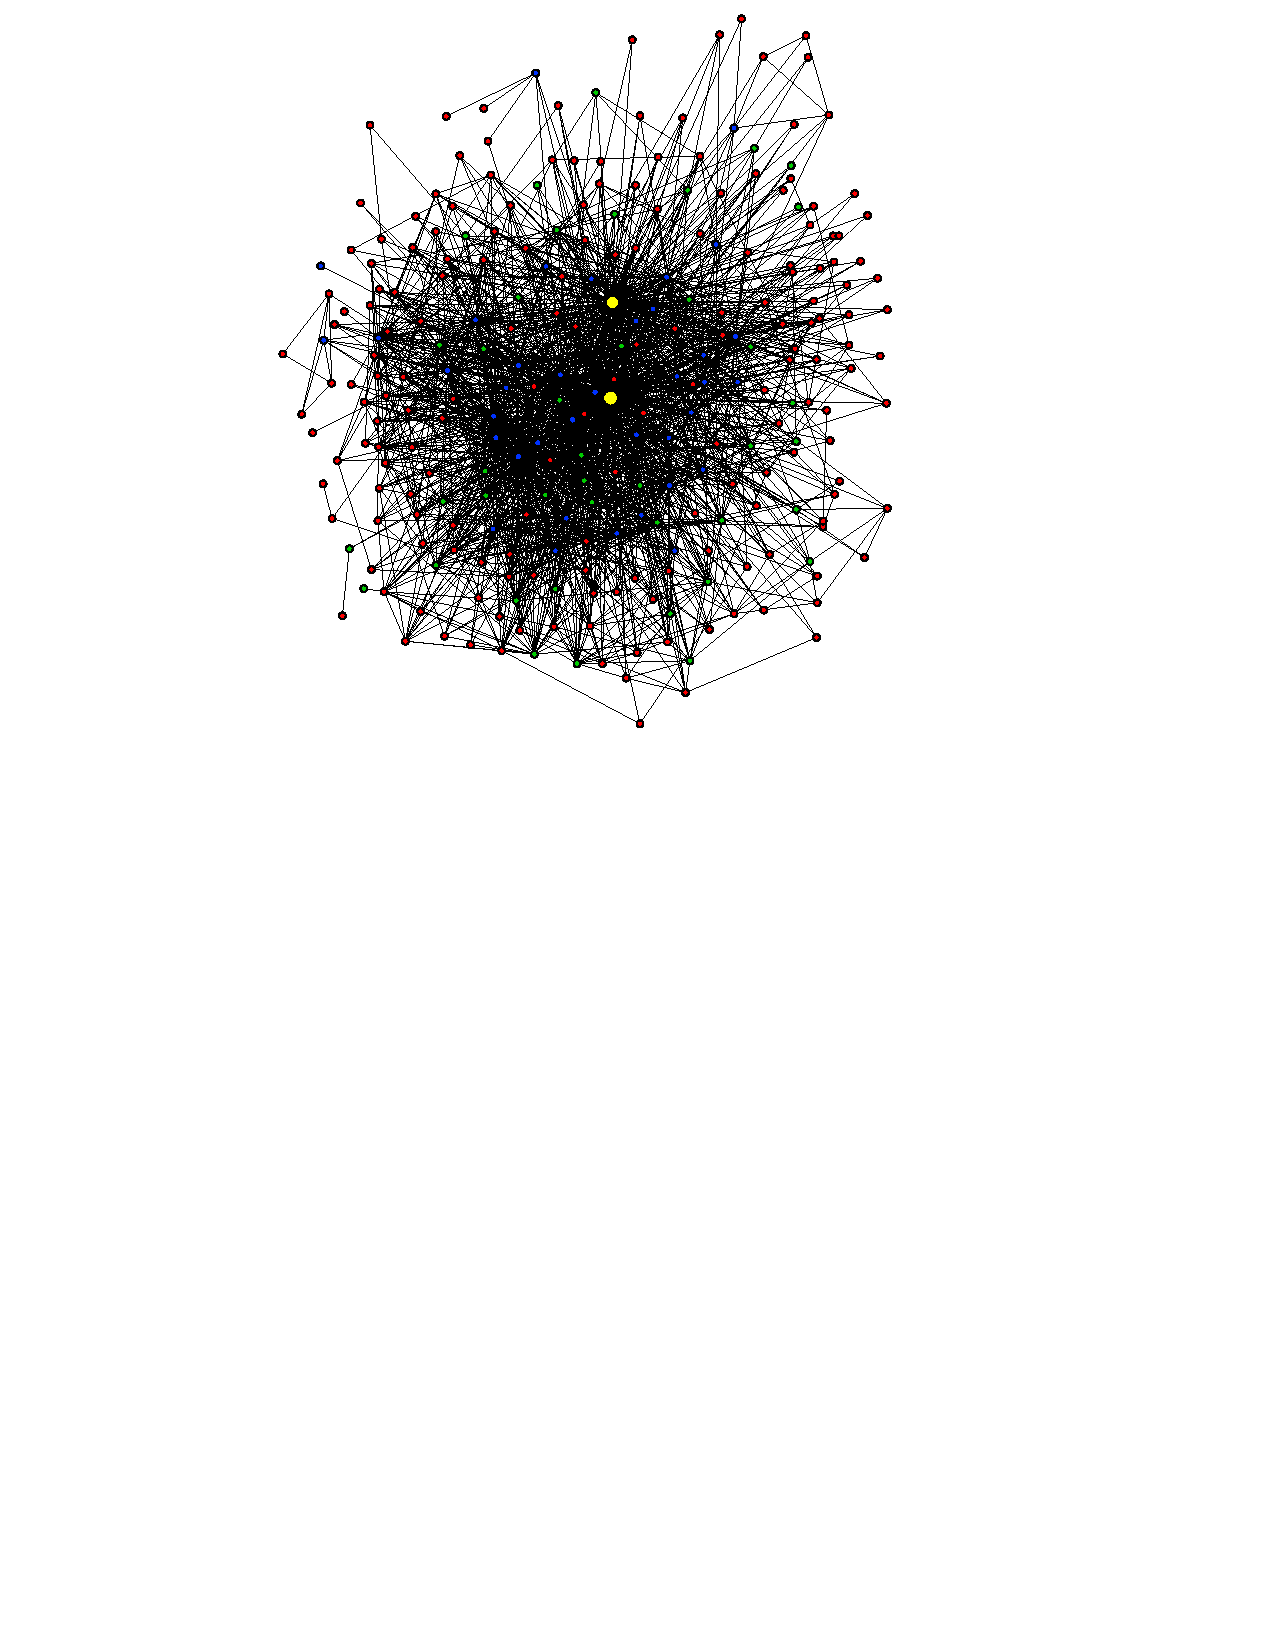
\includegraphics[scale=1.5]{images/label-prop-metagraph-20-narrow-cut.pdf}
  \caption{Struktur der Communities (Label-Propagation) (rot: Gr\"osse
    $<50$, gr\"un: Gr\"osse $<100$, blau: Gr\"osse < 1000, gelb:
    Gr\"osse > 1000).}
  \label{fig:metagraph-com-label}
\end{figure}

\begin{figure}[h]
  \centering
  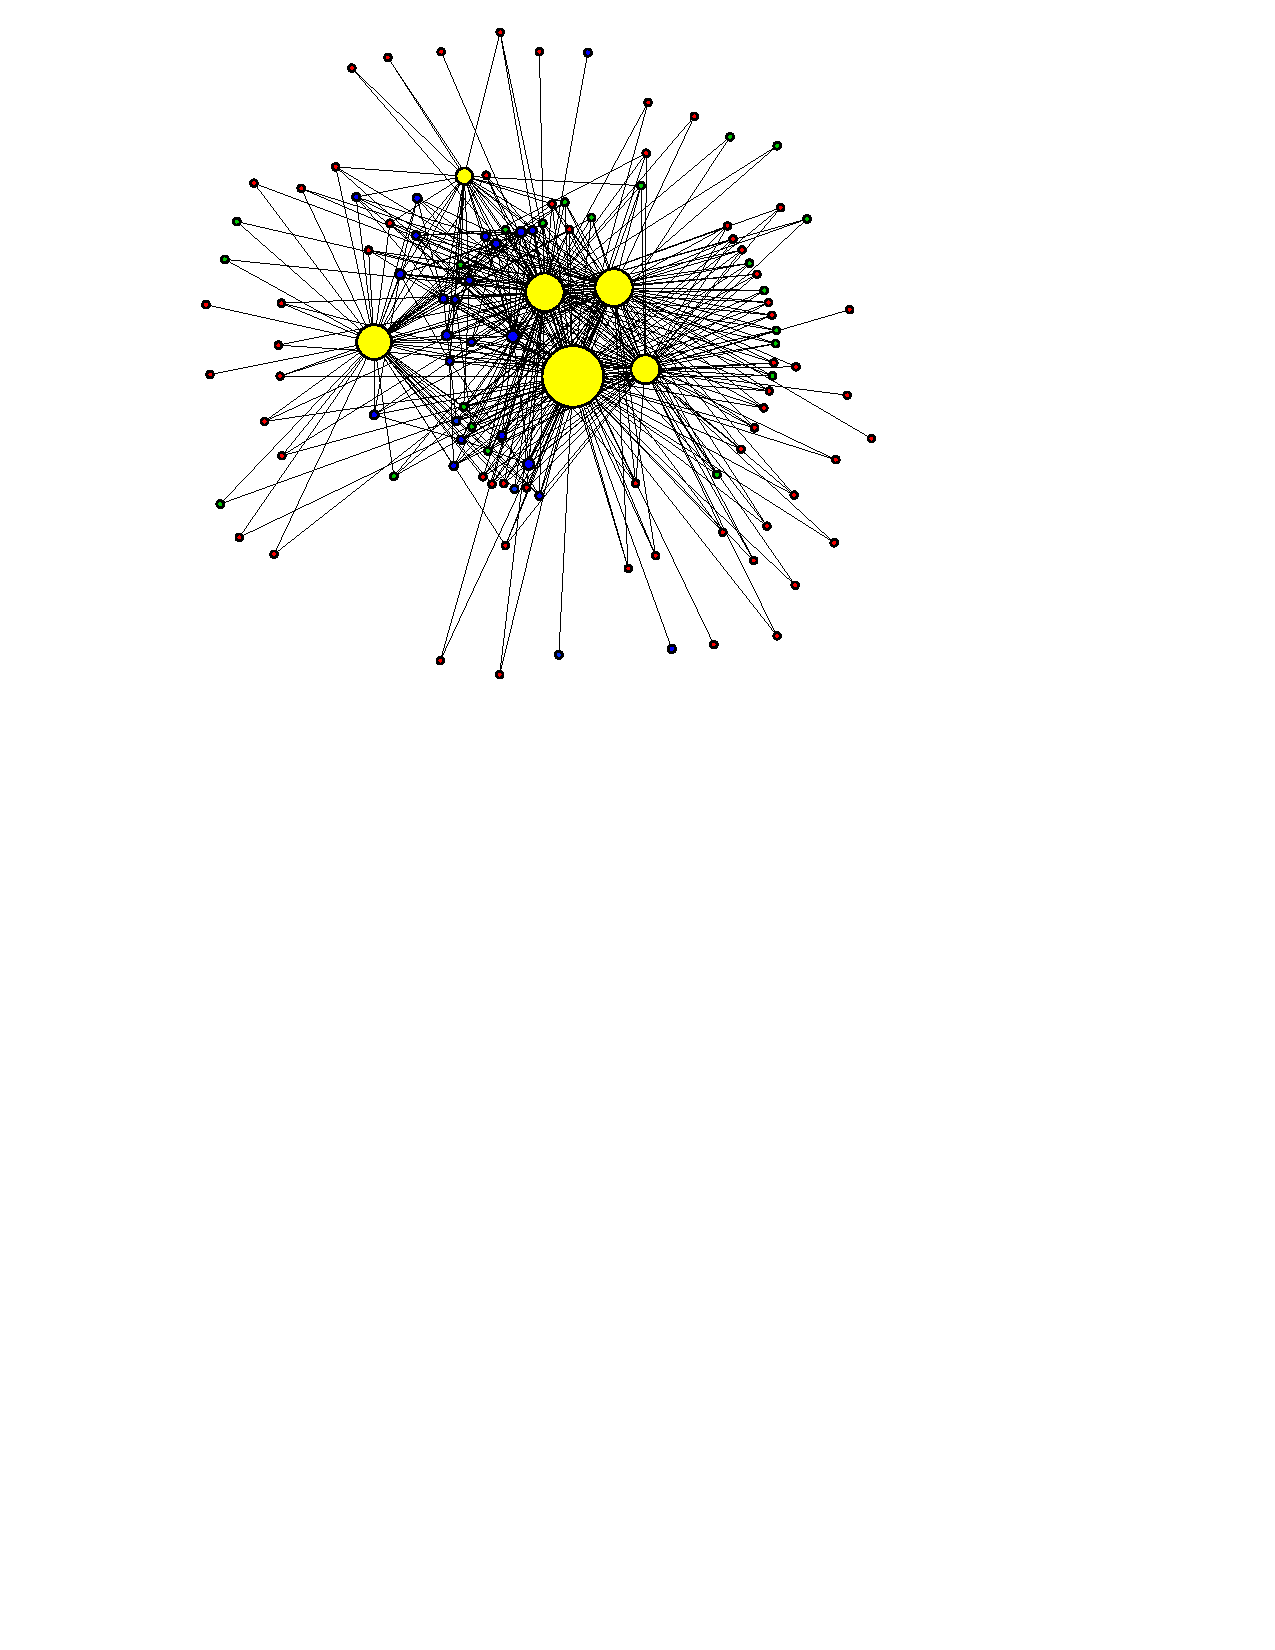
\includegraphics[scale=1.0]{images/fastmod-metagraph-20.pdf}
  \caption{Struktur der Communities (Fast Modularity) (Knotenf\"arbung
    wie in Abb.\ref{fig:metagraph-com-label})}
  \label{fig:metagraph-com-fastmod}
\end{figure}

\begin{figure}[h]
  \centering
  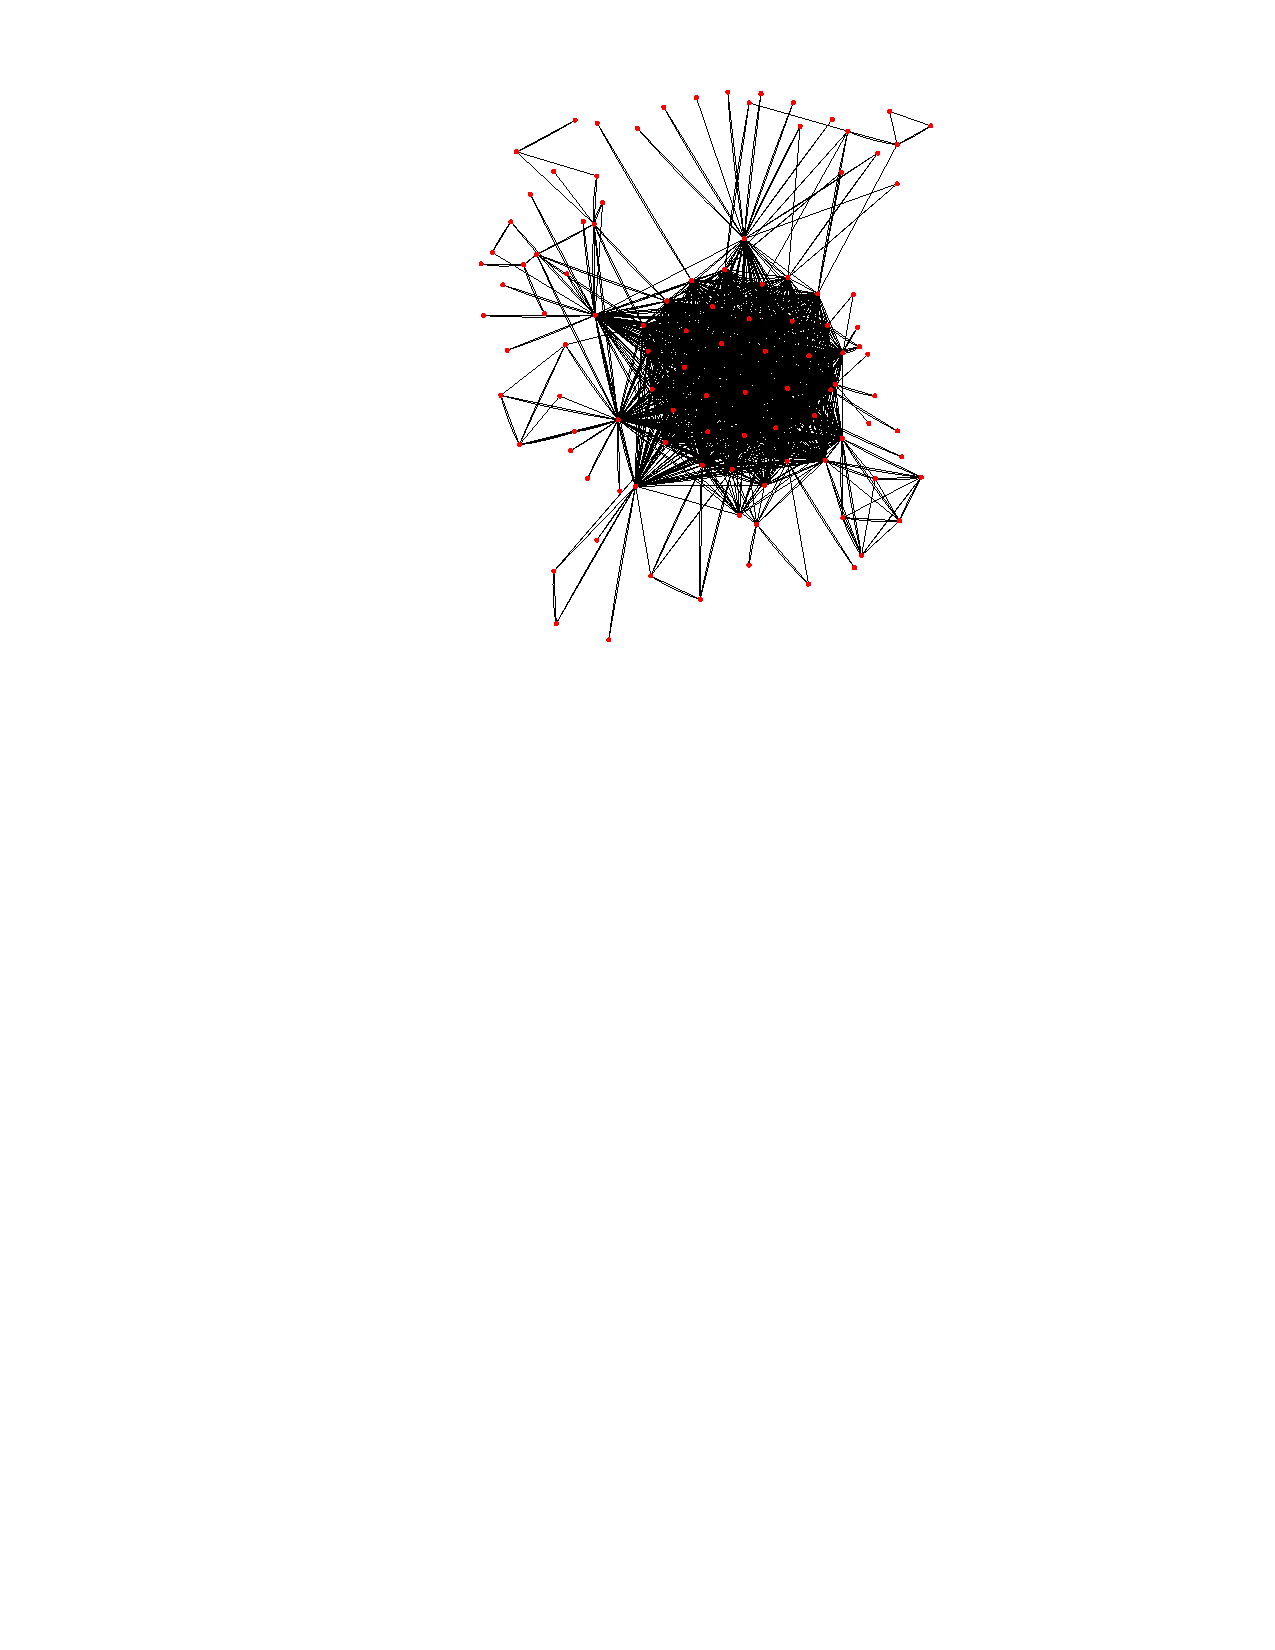
\includegraphics[scale=1.0]{images/subgraph-label-time-1077361cfa4161f22a2e4abb5ca89b8c1ad.pdf}
  \caption{foo}
  \label{fig:time-corr-com-normal}
\end{figure}

\begin{figure}[h]
  \centering
  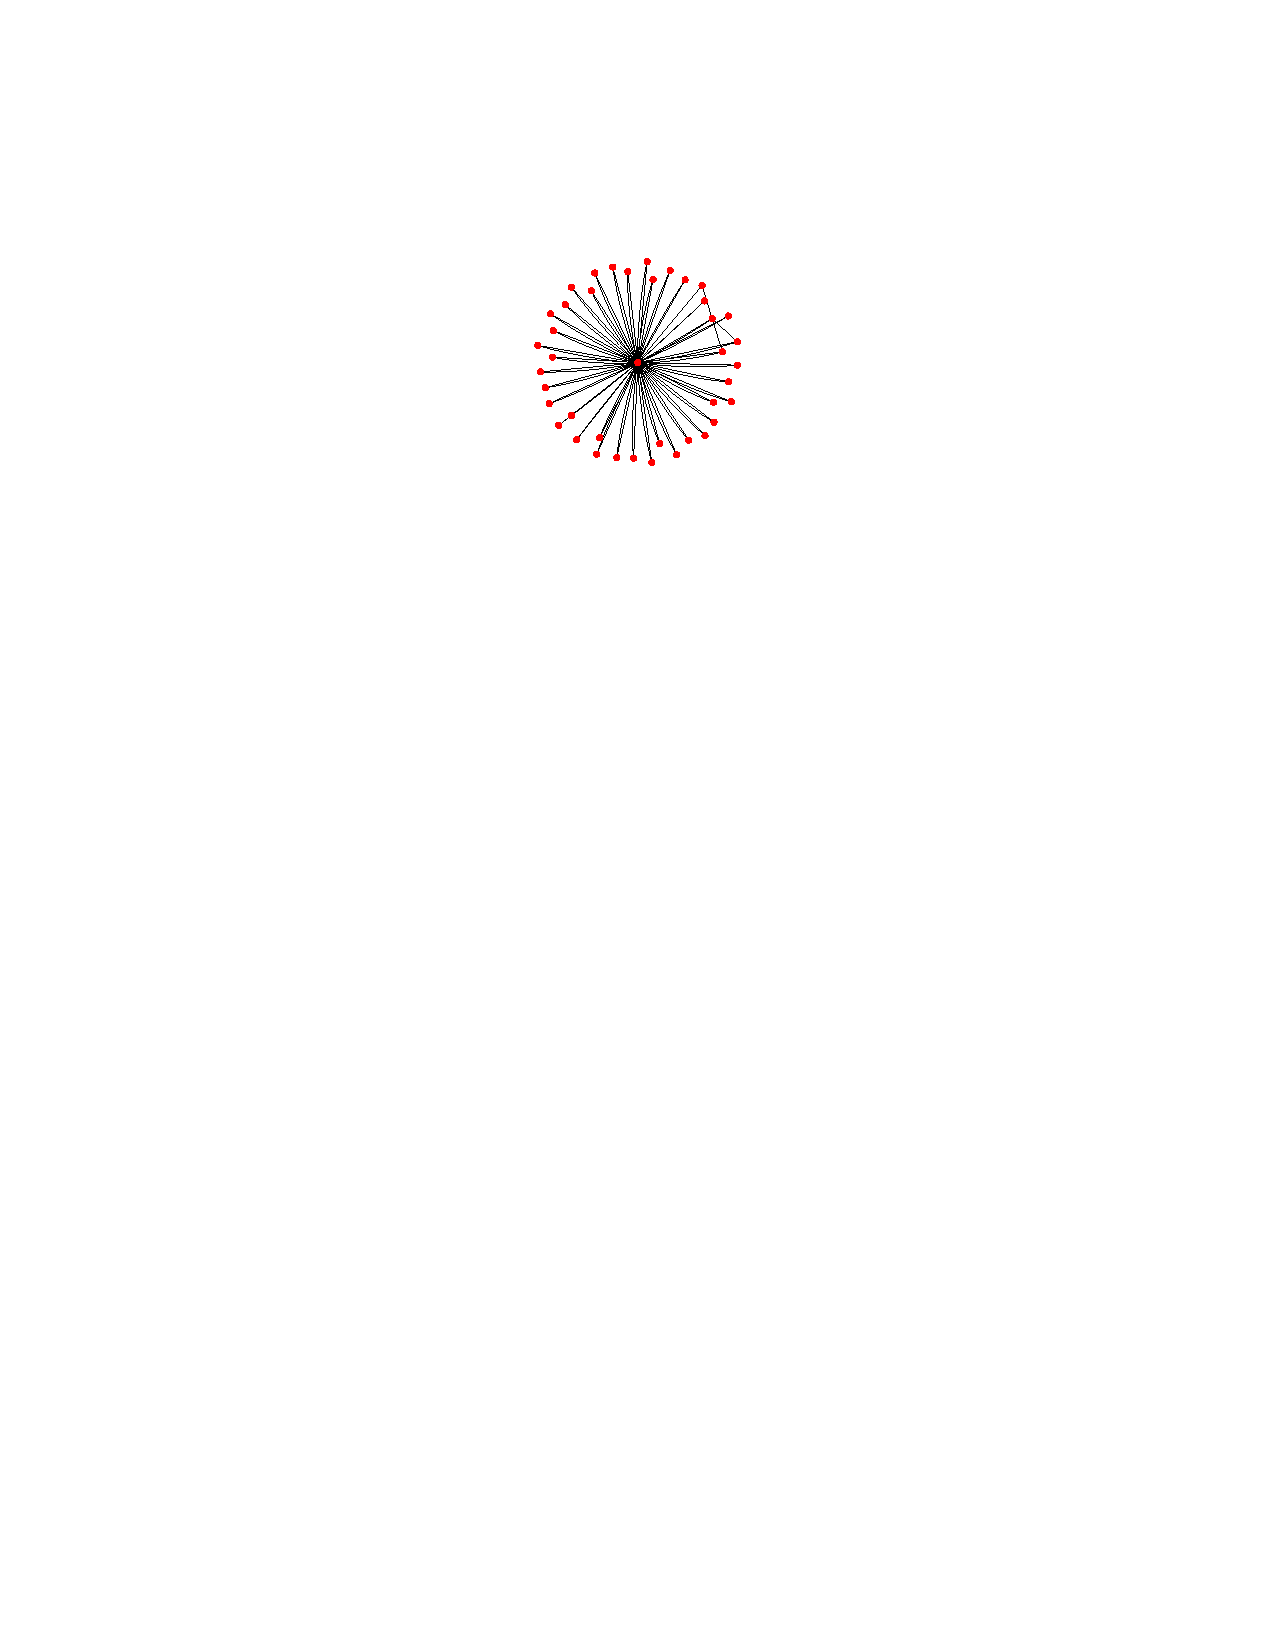
\includegraphics[scale=1.0]{images/label-subgraph-41-star-c222345bc5eb1f9eff80d58a81861974.pdf}
  \caption{foo}
  \label{fig:time-corr-com-star}
\end{figure}

\begin{figure}[h]
  \centering
  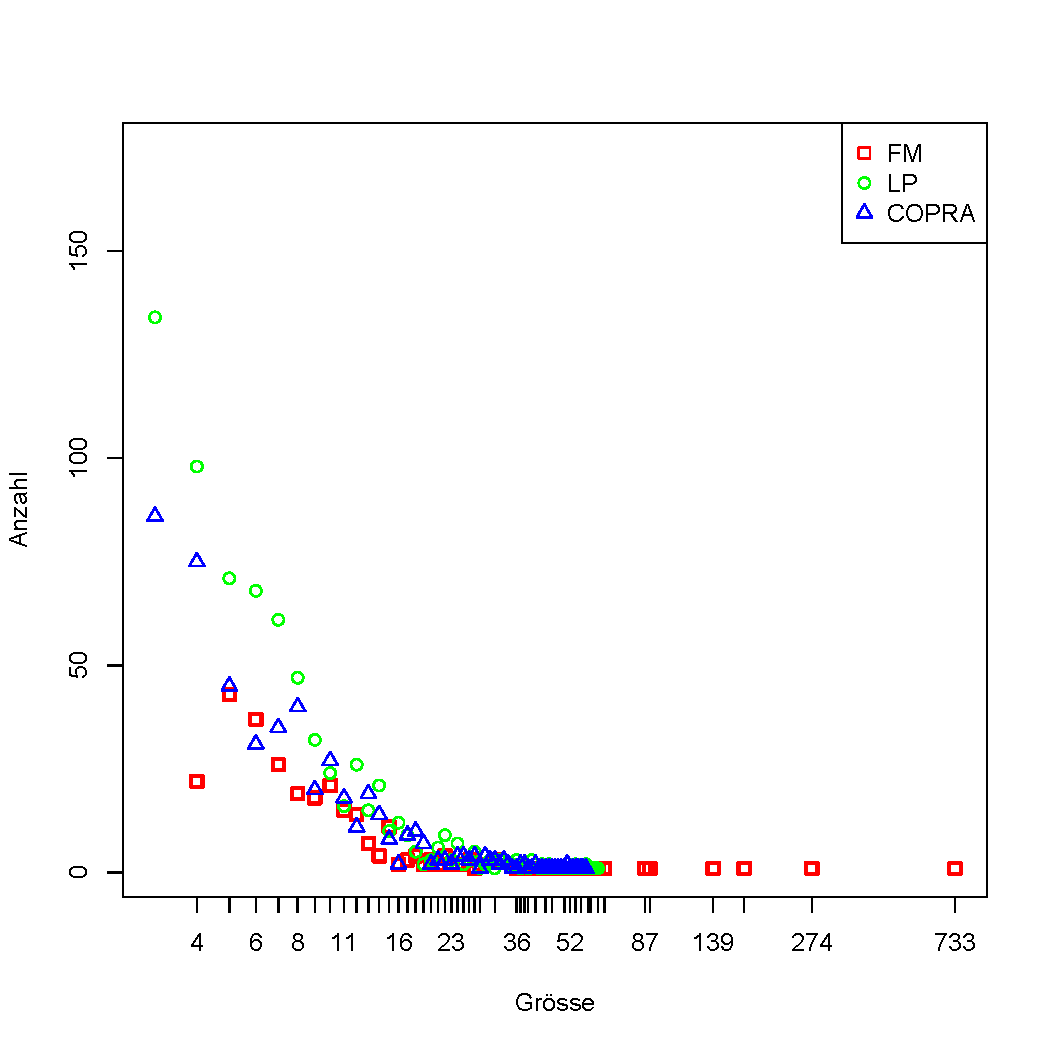
\includegraphics[scale=0.8]{images/tld_sure_dist.pdf}
  \caption{Zuweisung von Domains zu TLDs abh\"angig von der Community-Gr\"osse}
  \label{fig:tld-sure-ass-dist}
\end{figure}

\begin{figure}[h]
  \centering
  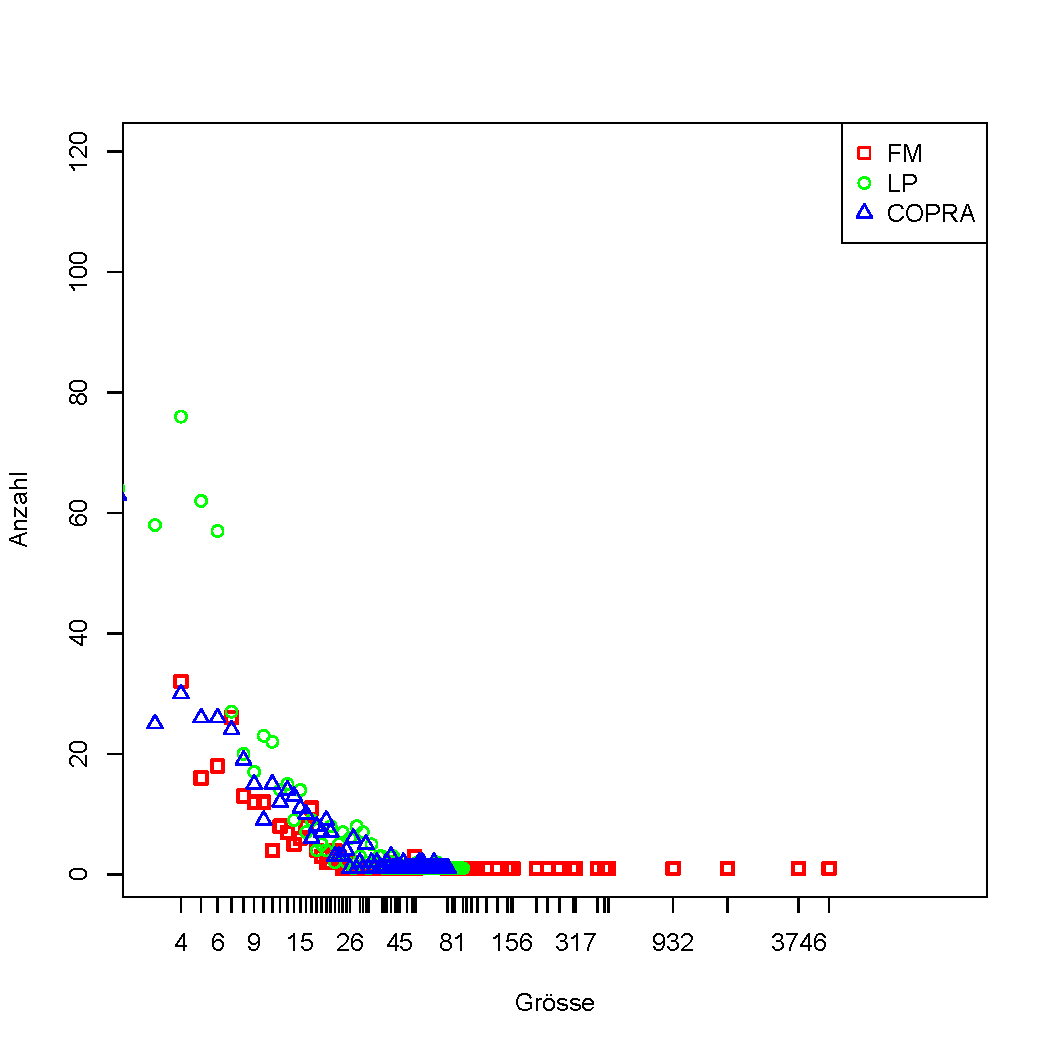
\includegraphics[scale=0.8]{images/tld_maybe_dist.pdf}
  \caption{Verteilung der Gr\"osse der von einer TLD dominierten Communities}
  \label{fig:tld-maybe-ass-dist}
\end{figure}

\begin{figure}[h]
  \centering
  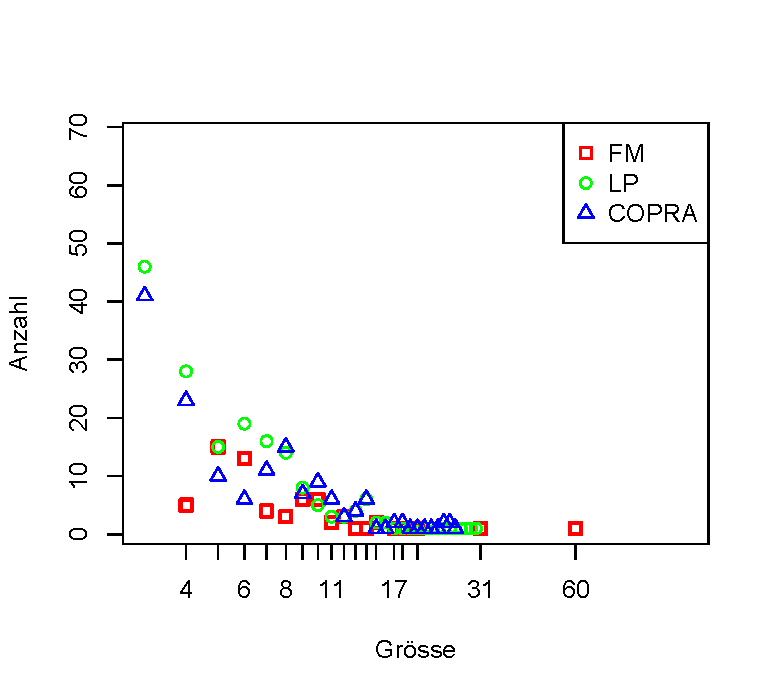
\includegraphics[scale=0.8]{images/sld_sure_dist.pdf}
  \caption{foo}
  \caption{Zuweisung von Domains zu SLDs abh\"angig von der Community-Gr\"osse}
  \label{fig:sld-sure-ass-dist}
\end{figure}

\begin{figure}[h]
  \centering
  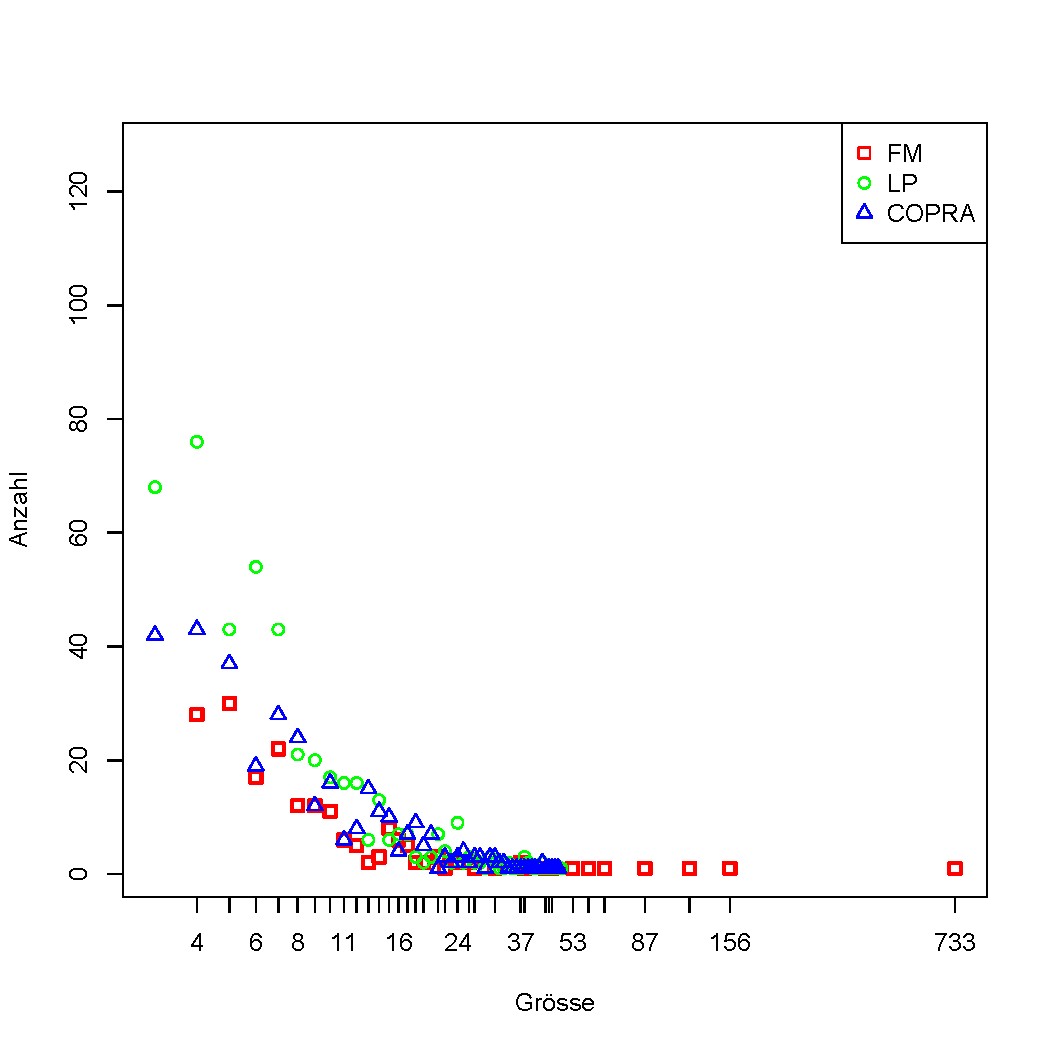
\includegraphics[scale=0.8]{images/sld_maybe_dist.pdf}
  \caption{Verteilung der Gr\"osse der von einer TLD dominierten Communities}
  \label{fig:sld-maybe-ass-dist}
\end{figure}

\begin{figure}[h]
  \centering
  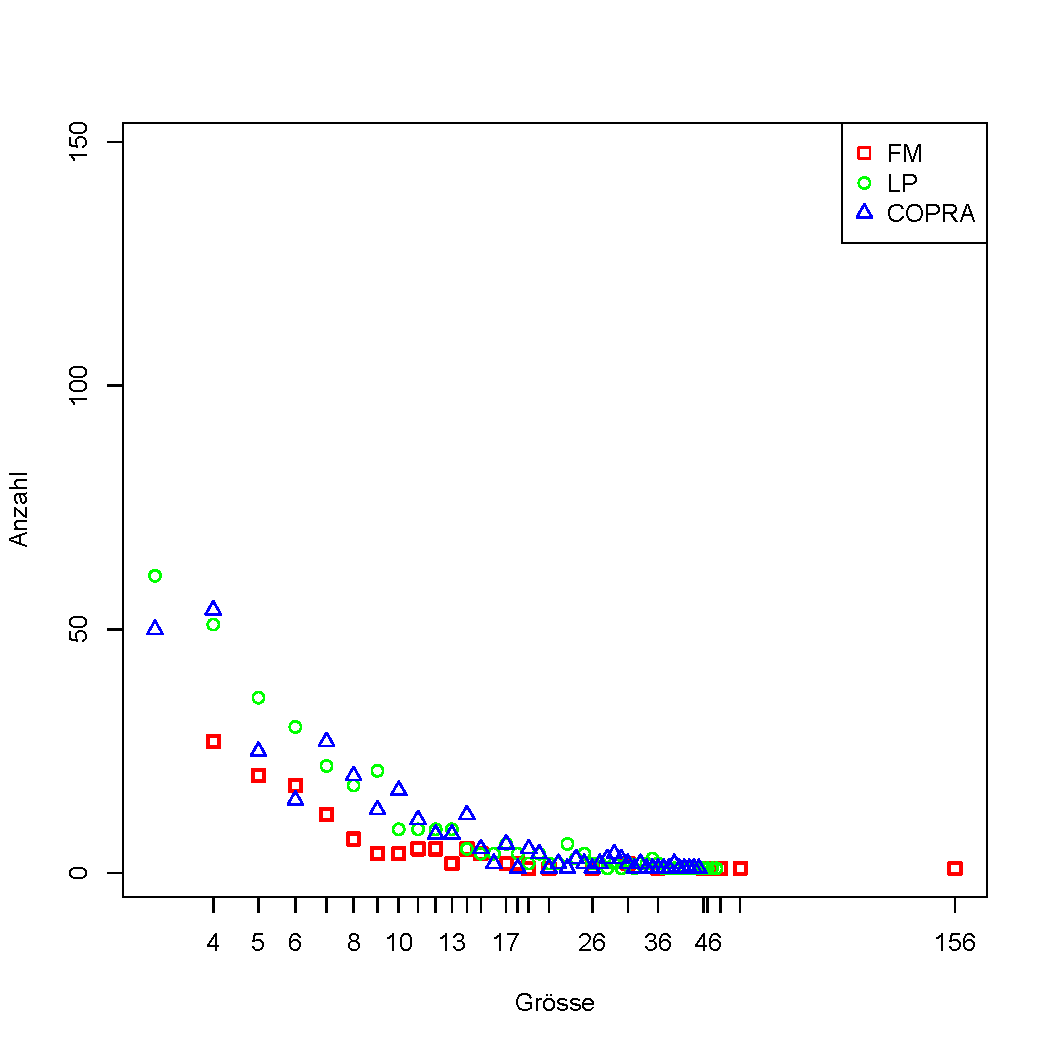
\includegraphics[scale=0.8]{images/time_corr_dist.pdf}
  \caption{Verteilung der Gr\"osse der Communities mit zeitlicher Korrelation}
  \label{fig:time-corr-dist}
\end{figure}


\subsection{Communities in gerichteten Graphen}
\label{sec:comm-gericht-graph}
erichteten Graphen definiert. Ebenso 

%%% Local Variables: 
%%% mode: latex
%%% TeX-master: "diplarb"
%%% End: 
